\customsection{House Manager}

Una vez descritos todos los componentes gráficos necesarios para realizar la aplicación, se implementaron los objetos de modelo, vista y controlador, basándose en los requerimientos descritos en la hoja ``requerimientos funcionales'' de la tabla \ref{tab0}. Para el desarrollo de estos componentes fueron necesarias diferentes condiciones técnicas que serán descritas en el siguiente apartado.

\subsection{Especificaciones técnicas}

La aplicación fue desarrollada utilizando el paradigma MVC, para ello, se organizo el proyecto en 3 carpetas: \textit{view, control y model}, donde todos los componentes y \textit{scripts} son gestionados desde un archivo principal. Debido a la naturaleza gráfica del proyecto y las limitaciones técnicas del hardware raspberry, se utilizó Python 2.7 para garantizar la compatibilidad de la mayor cantidad de sistemas operativos y librerías. 
Para el desarrollo de la aplicación fueron utilizadas las siguientes librerías:

\begin{itemize}
	\item \textbf{Paho-mqtt:} Esta librería se utilizó para establecer la comunicación con el bróker de Mqtt nativo de “Google Cloud Iot”.
	\item \textbf{Numpy, Scipy:} Estas listrerias fueron utilizadas para facilitar el procesamiento de vectores y mejorar el tiempo de procesamiento de los mismos.
	\item \textbf{Pyqtgraph:} Fue utilizada para gestionar el renderizado de las gráficas con el mejor valor posible de fotogramas por segundo. La necesidad de optimizar el componente grafico fue de importancia puesto que se desarrollaría sobre una tarjeta de computación de propósito específico (Raspberry).
	\item: \textbf{Http.client:} Esta librería fue utilizada para establecer una comunicación basada en solicitudes http con un ``endpoint'' del backend.
	\item: \textbf{Pyjwt, Cryptography:} Con esta librería se desarrolló la etapa de encriptación de datos adicional basada en \textit{Java Web Tokens}.	
\end{itemize}


Pensando en la escalabilidad del sistema, se definió un espacio para las ``aplicaciones'' adicionales donde se pudieran incluir nuevas rutinas de adquisición y control para dispositivos nuevos \ref{fig_6}. Como prueba de concepto se utilizó una rutina serial para adquirir el valor de khw acumulado en un contador eléctrico bifásico Inelca. Respecto a esta consideración de diseño se hablará más en el capitulo de ``pruebas y resultados''.
\vspace{0.5cm}\\

\begin{figure}[htbp]
	\centerline{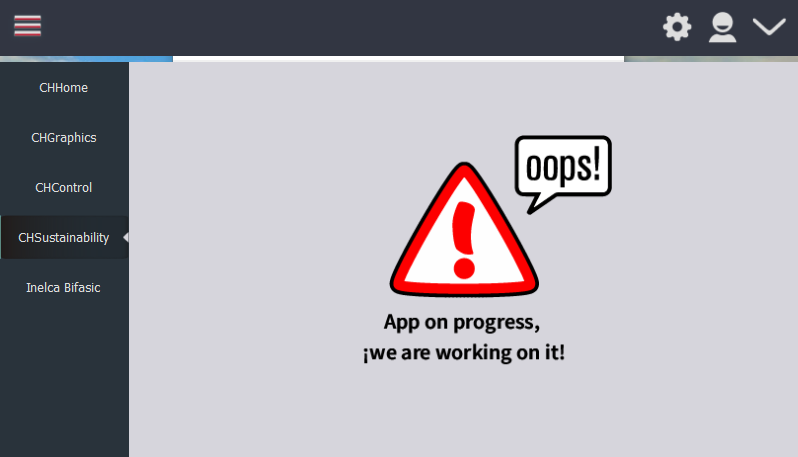
\includegraphics[width=8.5cm]{figuras/housemanager_newapp.png}}
	\caption{Visualización de la escalabilidad del sistema con una App no desarrollada por completo. Fuente: propia}
	\label{fig_6}
\end{figure}

En adición, se diagramó la experiencia de usuario de tal forma que el control y la medición de los dispositivos conectados a la tarjeta tuvieran el mismo ``costo de interacción'', es decir, que ambos estuvieran a la misma cantidad de clicks desde cualquier ventana del sistema. Por ende, todas las aplicaciones adicionadas en versiones futuras serán más fáciles de asimilar para el usuario.

\subsection{Requerimientos Funcionales}

Durante la etapa de conceptualización del proyecto de ingeniería que precede este documento se establecieron unos requerimientos funcionales con el fin de guiar el proceso de desarrollo. Este documento se puede ver el la tabla \ref{tab0}, y la implementación de cada requerimiento se puede observar a continuación:

\begin{figure}[htbp]
	\centerline{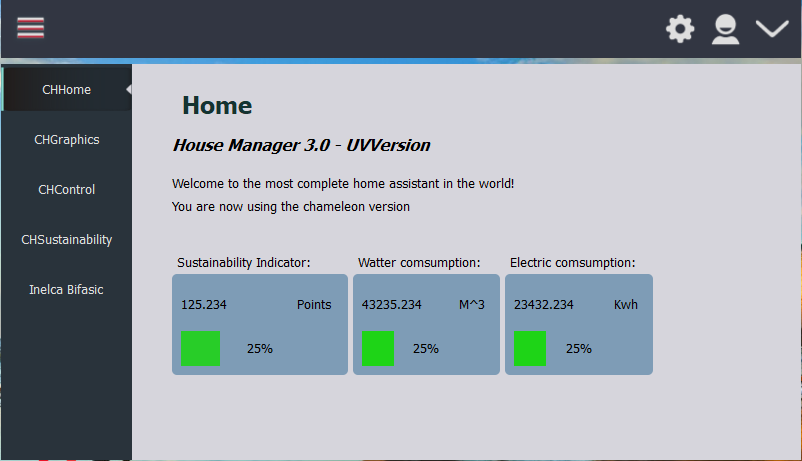
\includegraphics[width=8.5cm]{figuras/housemanager_home.png}}
	\caption{Escena del home del House Manager con barras de progreso para la indicación dinámica. Fuente: propia}
	\label{fig_7}
\end{figure}

\begin{enumerate}
	\item \textsl{``El sistema debe mostrar gráficamente la cantidad de agua y potencia consumida durante el día contrastándolas con un valor máximo recomendado'':} Para el desarrollo de esta funcionalidad se utilizó un componente gráfico tipo barra de progreso donde su 100 por ciento tenía como referencia la cantidad de agua recomendada para el número de personas presentes en la vivienda\ref{fig_7}. El número de personas presentes en la vivienda fue un dato ingresado manualmente por configuración inicial (sobre el sistema de configuración se hablará en los siguientes apartados de este capítulo).
	
	\item \textsl{``Por defecto el uso de las cargas eléctricas más significativas debe programarse durante los picos de generación en la casa, estos horarios podrán ser modificados bajo una advertencia de uso no eficiente'':} En miras de implementar esta funcionalidad se utilizó un elemento gráfico tipo calendario para configurar de manera individual las ventanas de activación de las cargas eléctricas en la vivienda\ref{fig_8}.
	\vspace{0.5cm}\\ 
	También, se consideró la opción de activación o desactivación inmediata de los circuitos; para ello se, implementó una rutina flexible que permitió ignorar las cargas eléctricas que el usuario había modificado manualmente (Esta rutina se nombró ``Scheduler Handler''), lo anterior únicamente durante 24 horas para no afectar el objetivo de sostenibilidad de la vivienda. 
	\vspace{0.5cm}\\
	Además, se utilizó la conexión Mqtt para accionar remotamente cualquiera de los circuitos localmente gestionados, en caso de recibir un mensaje de control para los circuitos el sistema también suspendiera por 24 horas la acción del ``Schedule Handler''.
	\item: \textsl{``El usuario debe poder acceder a la información medida en tiempo real'':} Para la implementación de este requerimiento se creo una ventana gráfica con la capacidad de mostrar el valor de la medida del sensor con un tiempo de muestreo entre 1 y 50 Hertz. Teniendo en cuenta lo anterior, el medidor debe ser capaz de almacenar el valor de consumo eléctrico y de agua internamente. Tal como lo hace el contador eléctrico bifasico de Inelca con el que se realizaron las pruebas.
	\vspace{0.5cm}\\
	Si el usuario lo desea, puede cambiar el numero de puntos y la frecuencia de muestreo de manera inmediata, moviendo las barras deslizables. Ademas, puede guardar los datos mostrados en la gráfica en el formato de excel presionando el boton ``save to file''.
	\item: \textsl{``El sistema debe poder comunicarse con una base de datos que represente todas las variables y el estado de los circuitos de la vivienda'':} Para la implementación de este requerimiento se creo un ``endpoint'' en el servicio de \textit{backend} con la capacidad de hacer consultas de históricos a la base de datos (Un ``endpoint'' es un url web gestionado por un backend en el cual se pueden realizar solicitudes Http). La solución tiene este comportamiento puesto que la aplicación del cliente final no debe tener ningún tipo de credencial para el acceso a la información directamente, con una capa de procesamiento se pueden integrar este tipo de solicitudes con el mismo sistema de encriptacion del broker de Mqtts (para más información de los endpoints y la rutina de encriptacion vease el capitulo \textit{backend}).
\end{enumerate}


\begin{figure}[htbp]
	\centerline{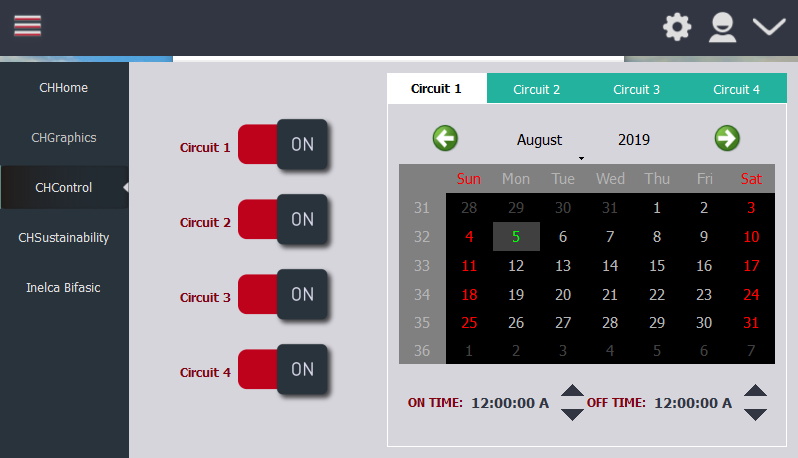
\includegraphics[width=8.5cm]{figuras/housemanager_control.png}}
	\caption{Escena de control del House Managern con sus calendarios. Fuente: propia}
	\label{fig_8}
\end{figure}

\subsection{Funciones adicionales}

En adición a los requerimientos funcionales, se añadieron funciones a la conceptualización de diseño original para mejorar el funcionamiento de la plataforma y la experiencia de usuario. Dentro de estas funciones podemos encontrar la configuración del sistema, la posibilidad de guardar localmente para no perder la información adquirida, etc. Para comprender mejor estas funciones adicionales, serán descritas a continuación:

\begin{enumerate}
	\item \textbf{Handler remoto:} Esta característica le permite al sistema cambiar de manera automática entre el modo remoto y el modo local para no perder información en ningún momento del reporte de datos. En caso de la caída repentina de la red, el programa es capaz de cambiar al modo local sin la perdida de ningún dato. También, es capaz de entender cuando el usuario desea que el dispositivo funcione permanentemente de manera local o cuando el sistema vuelve a estar nuevamente conectado a la red. Los datos que son guardados de manera local se almacenan en la carpeta personal del usuario, en archivos de excel, y son creados por dia con la fecha como nombre. Teniendo en cuenta lo anterior, el nivel de autonomia local depende exclusivamente de la memoria en el disco duro; para la Raspberry fueron aproximadamente 10 GB de las 16 disponibles en la memoria micro SD.
	
	\item \textbf{Sistema de almacenamiento local:} Con esta característica el House Manager puede almacenar todos los datos adquiridos en una hoja de Excel generando archivos organizados por días. También es capaz de almacenar en un archivo diferente los datos presentes en la gráficas teniendo en cuenta el día de adquisición. \ref{fig_9}.
	\begin{figure}[htbp]
		\centerline{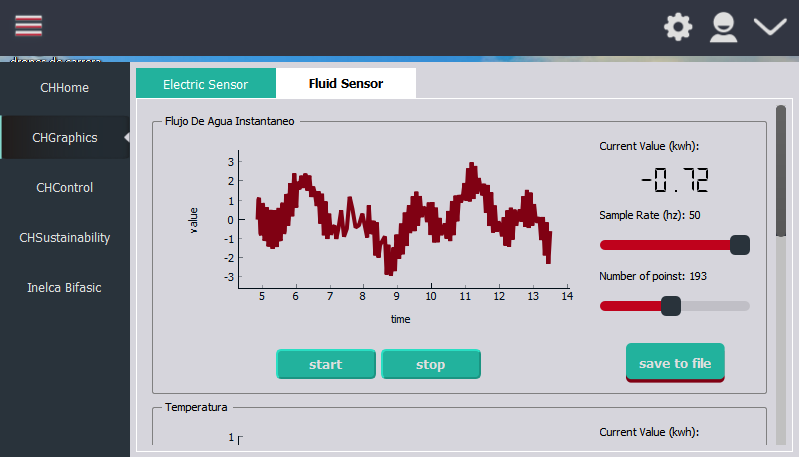
\includegraphics[width=8.5cm]{figuras/housemanager_measure.png}}
		\caption{Escena de medición del House Manager, con su respectivo panel para guardar los datos. Fuente: propia}
		\label{fig_9}
	\end{figure}

	\item \textbf{Ajustes de configuración} Esta es una característica que incluye una ventana adicional donde se configuran los aspectos concernientes al sistema en general\ref{fig_10}. Los aspectos configurables del sistema son: La frecuencia en segundos con la que se reportan los datos al servidor, el costo del kilo watt hora, el costo del metro cubico de agua, el día de notificación del correo (ver función ``Notificación automática''), el modo de funcionamiento (remoto o local) y el nombre de la ubicación (este nombre es opcional y sirve para administrar los diferentes dispositivos desde la perspectiva del backend).
	\begin{figure}[htbp]
		\centerline{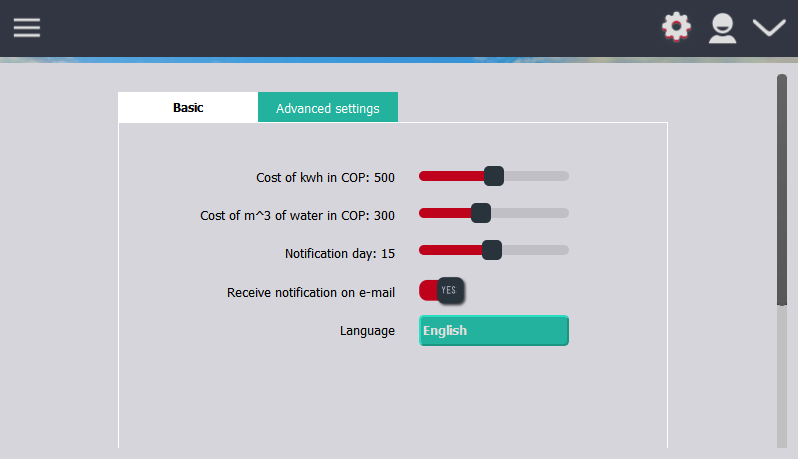
\includegraphics[width=8.5cm]{figuras/housemanager_config.png}}
		\caption{Escena de configuración del dispositivo House Manager. Fuente: propia}
		\label{fig_10}
	\end{figure}

	\item \textbf{Notificación Automática:} Para el correcto desarrollo de esta función se compró el dominio \href{www.alfagenos.com}{www.alfagenos.com} para recibir las notificaciones desde el remitente de correo: notificaciones@alfagenos.com. Esta notificación tendrá lugar dependiendo de la configuración establecida e indicara el gasto en pesos del consumo eléctrico y de agua hasta la fecha establecida en la configuración. También notificará los gastos  energéticos en horarios adicionales al pre establecido por la configuración del Solar Decathlon.
	
	\item\textbf{Autenticación usando google:} Para desarrollar esta funcionalidad se utilizó la api de autenticación de google y se creo una escena aparte para la visualización del usuario \ref{fig_11}.
	\begin{figure}[htbp]
		\centerline{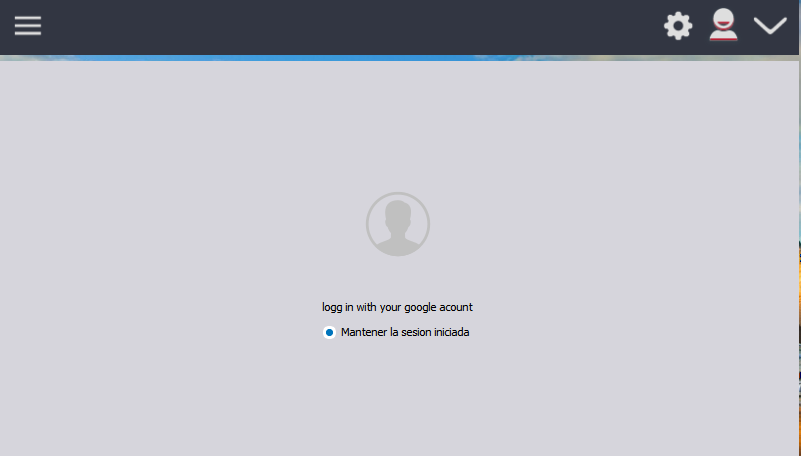
\includegraphics[width=8.5cm]{figuras/housemanager_user.png}}
		\caption{Escena para el inicio de sesión del House Manager. Fuente: propia}
		\label{fig_11}
	\end{figure}
	
	\item \textbf{Doble nivel de encriptación:} Debido a las exigencias de los servidores de Google se implementaron 2 capas de seguridad de encriptación para la  comunicación de la aplicación con el backend. La primera capa es de tipo Tls y opera para cualquier producto de google, inclusive las operaciones realizadas por los navegadores. La segunda se desarrolló usando encriptación ``RS256'' a través de Jwt.
\end{enumerate}

\subsection{Algoritmos Utilizados}

Para cumplir con algunos requerimientos funcionales y algunas funciones adicionales, fue implementar hilos de proceso en segundo plano que se encargaron de tareas que no eran sensibles a pequeños cambios en la frecuenciade ejecucion. Los algoritmos utilizados en estos hilos de programa, comparten la información de toda la aplicación a través de los 3 objetos principales: el controlador la vista y el modelo. Estos algoritmos o programas ocurren en segundo plano y no representan una carga significativa para el CPU ni se comportan de manera determinista respecto a los tiempos de ejecución establecidos para los mismos. 

\subsubsection{Scheduler Handler}
Este Hilo es el encargado de verificar y mantener el estado de los circuitos según ha sido configurado en la ventana del horario de manera automatica. Este hilo de programa es capaz de discernir los circuitos que se han activado de manera manual desde la aplicación móvil o desde la interfaz de escritorio. Ante un evento de estos (manual), la influencia de la ventana de activacion o desactivacion automatica se desactiva por 24 horas y el circuito entra en un modo manual por 24 horas.
.
\subsubsection{Remote Mode Handler}
Este hilo de programa está encargado de verificar el estado de la conexión con el servidor para cambiar el modo de almacenamiento de la información, si es necesario. Si el dispositivo se desconecta, el sistema de almacenamiento cambia a la memoria local y si vuelve la conexión el handler es capaz de conectarse automáticamente al broker web para reportar los datos nuevamente, sin perdida de información.

\subsubsection{Mail Notification Handler}

Este hilo es el encargado de verificar la fecha y realizar las notificaciones correspondientes al consumo eléctrico, el consumo de agua y el indicador de sostenibilidad. También, lleva el registro del consumo generado por fuera de los horarios recomendados por el Solar Decathlon.

\subsubsection{Data Report Handler}

Esta rutina es la encargada de reportar automáticamente los valores medidos y almacenados en las gráficas, esta rutina almacena datos con una periodicidad que va desde  cada segundo hasta cada 5 minutos. Como aclaración, cada vez que se reportan los datos de las gráficas, no se toman en cuenta todos los datos intermedios, por ende hay una perdida para variables de medición con una granularidad mayor a 1 segundo. En la figura \ref{fig_34} se puede observar que el periodo ``T1'' corresponde al tiempo de muestreo de alta granularidad a partir de la cual se grafican los datos en tiempo real en la ventana de medición; por otro lado, el periodo ``T2'' corresponde al tiempo de muestreo a partir del cual se guardan los datos en el servidor o en memoria.
\begin{figure}[htbp]
	\centerline{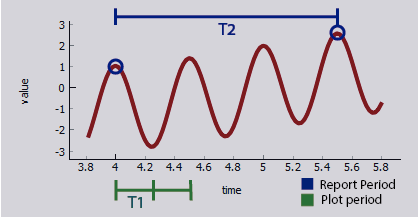
\includegraphics[width=8.5cm]{figuras/graph_explanation.png}}
	\caption{Descripción de los tiempos de muestreo utilizados en el sistema de adquisición. Fuente: propia}
	\label{fig_34}
\end{figure}

\subsubsection{Indicator Handler}

Esta es la rutina que se encarga de monitorear el estado de consumo eléctrico y de agua para modificar los valores de los indicadores de la ventana de inicio. Así como también, calcular el valor del indicador de sostenibilidad utilizando exclusivamente en el consumo eléctrico y de agua.


 
